% TO COMPILE %

%%%%%%%%%%                             %%%%%%%%%%
%%%%%%%%%% AUTO INSERTION D'UNE ENTETE %%%%%%%%%%
%%%%%%%%%%                             %%%%%%%%%%
%%%%%%%%%%     POUR UN FICHIER TEX     %%%%%%%%%%
%%%%%%%%%%                             %%%%%%%%%%

%%%%%%          %%%%%%
%%%%%% PACKAGES %%%%%%
%%%%%%          %%%%%%

\documentclass[a4paper]{article}
\usepackage{fullpage}
\usepackage[utf8]{inputenc}
\usepackage[francais]{babel}
\usepackage{graphicx}
\usepackage{listings}
\usepackage{color} 
\usepackage{enumerate}
\usepackage{amsfonts}
\usepackage{amssymb}
\usepackage{amsmath}
\usepackage{wasysym}
\usepackage{chemarrow}
\usepackage[colorlinks=true, urlcolor=blue]{hyperref}

%%%%%%              %%%%%%
%%%%%% MISE EN PAGE %%%%%%
%%%%%%              %%%%%%


%%%%% Marges %%%%%
%\addtolength{\textwidth}{3cm}
\addtolength{\oddsidemargin}{-1cm}
%\textheight=22cm % longueur utile de la page
%\topmargin=2cm % marge haute
%\headsep=20pt % séparation 20 points entre entête et texte
%\footskip=20pt % idem séparation pied de page

%%%%% Entetes et Enpieds de pages %%%%%
\usepackage{fancyhdr}
\pagestyle{fancy}
\lhead{\footnotesize{\textit{Kuntz Fabien}}}
\rhead{\footnotesize{\textit{Techniques de Vérification - Frédéric
Herbreteau}}}

%%%%% Numérotation sections %%%%
\setcounter{secnumdepth}{3}
\setcounter{tocdepth}{3}

%%%%% Types enumerate %%%%%
\renewcommand{\labelenumi}{-}
\renewcommand{\labelenumii}{$\bullet$}
\renewcommand{\labelenumiii}{$\star$}
\renewcommand{\labelenumiv}{\_}

%%%%% Titre %%%%%
\newlength{\larg}
\setlength{\larg}{14.5cm}

%%%Zone de Code%%%
\definecolor{gray}{gray}{0.86}  

\lstset{numbers=left, tabsize=2, frame=single, breaklines=true,
basicstyle=\ttfamily,numberstyle=\tiny\ttfamily, framexleftmargin=13mm,
backgroundcolor=\color{gray}, xleftmargin=14mm} 

\newsavebox{\fmbox}
\newenvironment{fmpage}[1]{\begin{lrbox}{\fmbox}\begin{minipage}{#1}}{\end{minipage}\end{lrbox}\fbox{\usebox{\fmbox}}}


%%%%%%          %%%%%%
%%%%%% DOCUMENT %%%%%%
%%%%%%          %%%%%%


\begin{document}


%%%%% Page de présentation %%%%%
\thispagestyle{empty}

\setlength{\unitlength}{1in}

%%%%% Image de fond %%%%%
% \begin{picture}(0,0)
% \put(0.2,-7){\includegraphics[width=\textwidth]{images/bx1_trans.eps}}
% \end{picture}

\begin{flushright}
 \noindent {\rule{\larg}{0.5mm}}
\end{flushright}
\vspace{7mm}
\begin{flushright}
 \Huge{\bf Algorithmes du Monde Réel} \\
 \Huge{\bf Projet} \\
 ~\\
 \huge{Partie 1 - Réductions}\\
 % \Large{\bf{\emph{Fabien Kuntz}}}
\end{flushright}
\vspace{7mm}
\begin{flushright}
 {\rule{\larg}{0.5mm}}
\end{flushright}
\vspace{2mm}
\begin{flushright}
 \large{\bf Professeurs : M. Zeitoun, A. Muscholl, C. Gavoille} \\
 ~\\
 \large{Master 2 Informatique}\\
 ~\\
 % \today
 \vspace{10cm}
 \large{Ludovic Brochard, Fabien Kuntz, Védrenne Benoît}
{\rule{\larg}{0.5mm}}
\end{flushright}

\newpage

\addtolength{\oddsidemargin}{1cm}

%%%%% Table des matières %%%%%
\thispagestyle{empty}
\tableofcontents
\newpage

\setcounter{page}{1}


%%%%%%              %%%%%%
%%%%%% ZONE DE CODE %%%%%%
%%%%%%              %%%%%%

 %==============================================================================
 \begin{frame}
  \frametitle{Le projet}
  
  \begin{block}{Principe}
   \begin{itemize}
    \item Deux robots : Maître et Esclave
	  \uncover<2->{
    \item Robot Maître : capteurs et moteurs}
	  \uncover<3->{
    \item Robot Esclave : seulement moteurs}
	  \uncover<4->{
    \item Maître communique les ordres à l'Esclave par Bluetooth}
	  \uncover<5->{
    \item Esclave : pas de décision}
   \end{itemize}
  \end{block}

  \uncover<6->{
  \begin{block}{But}
   \begin{itemize}
    \item Accomplir une mission non triviale mettant en jeu les deux robots
	  \uncover<7->{
    \item Vérifier cette mission en modélisant en Altarica}
    \uncover<8->{
    \item Etudier la possibilité d'une generation de code automatique}
   \end{itemize}
  \end{block}
  }

 \end{frame}

 \section{Choix}
 Dans cette partie, nous allons présenter quelques uns des choix que
 nous avons faits concernant notre programme.

  \subsection{Langage}
  Nous avions le choix de faire ce projet en \emph{C} ou en
  \emph{C++}. Nous avons choisi \emph{C++} pour la simple raison que des
  structures de données intéressantes (notamment \emph{vector}) sont
  déjà présentes dans ce langage alors qu'elles ne le sont pas dans le
  langage \emph{C}.
  
  \subsection{Structure de données}
  Dans ce projet, nous avions à faire le choix d'une structure de
  données pour représenter les graphes. Nous avons suivi les conseils en
  décidant d'utiliser des listes d'adjacence.

  Plusieurs raisons nous ont poussés à utiliser les listes d'adjacence
  plutôt que d'autres structures\footnote{Il n'y a ici, pas de bon choix
  à proprement parler, le mieux serait de faire au cas par cas (nous en
  parlerons dans le bilan du rapport).} :
  \begin{enumerate}
   \item La liste d'adjacence est une des structures qui prend le moins
	 de place en mémoire car elle ne stocke que les sommets voisins
	 (contrairement à une matrice d'adjacence par exemple).
   \item La liste d'adjacence est très efficace lorsqu'on a à
	 considérer la liste des voisins des sommets (c'est son essence
	 même), ce qui est le cas pour nos réductions.
   \item La liste d'adjacence est évidemment plus efficace que n'importe
	 quelle structure d'incidence lorsqu'il s'agit de considérer les
	 sommets plutôt que les arêtes.
  \end{enumerate}

    \subsection{Dépendances et Relations}
  Le programme est simple d'utilisation puisqu'il suffit de le lancer
  avec un fichier d'entrée de type graphe issu du programme
  \emph{gengraph} de
  \emph{C. Gavoille}\footnote{\url{http://dept-info.labri.fr/~gavoille/gengraph.c}}
  ainsi qu'avec le numéro du problème et éventuellement des paramètres
  propres au problème.\\
  Le programme se déroule de la manière suivante :
  \begin{enumerate}
   \item Le fichier de graphe est lu à partir du fichier de graphe
	 fourni. 
   \item Selon le problème sélectionné, on lance la réduction
	 correspondante. 
   \item Une formulation en clauses de type \emph{CNF} est créée et
	 envoyée au \emph{SATSolver} \emph{Minisat}. 
   \item \emph{Minisat} crée une solution (si cela est possible).
   \item La solution fournie est analysée afin de pouvoir être
	 traitée. De cette manière, nous connaissons la solution au
	 problème voulu sur le graphe passé en paramètre. 
  \end{enumerate}
  
  En décrivant l'exécution du programme de cette façon, il est aisé de
  voir apparaître les relations entre les modules de notre programme.

  La fonction principale \emph{main}, contenue dans \emph{Solve.cpp},
  joue le rôle du tri des arguments et de construction du
  graphe. Ensuite, est appelée la réduction voulue, contenue dans les
  fichiers portant le nom d'un problème (ou leur abréviation). Une fois
  la réduction effectuée par ce fichier, celui-ci appelle un ``parser''
  pour \emph{Minisat} (dans \emph{MinisatBuilder.cpp}) qui gère le fait
  d'écrire un fichier d'entrée à \emph{Minisat}, de lancer le
  \emph{SAT-Solver} et d'analyser sa sortie. Une fois la sortie
  analysée, une assignation des variables est donnée. Celle-ci nous
  permet alors de fournir l'ensemble des arêtes ou sommets nécessaire
  définissant une solution du problème donné sur le graphe donné.\\

  Voici un graphe représentant simplement les relations entre les
  différentes parties du programme (fig.\ref{grapheExec} page
  \pageref{grapheExec}).
  \begin{figure}[!ht]
   \begin{center}
    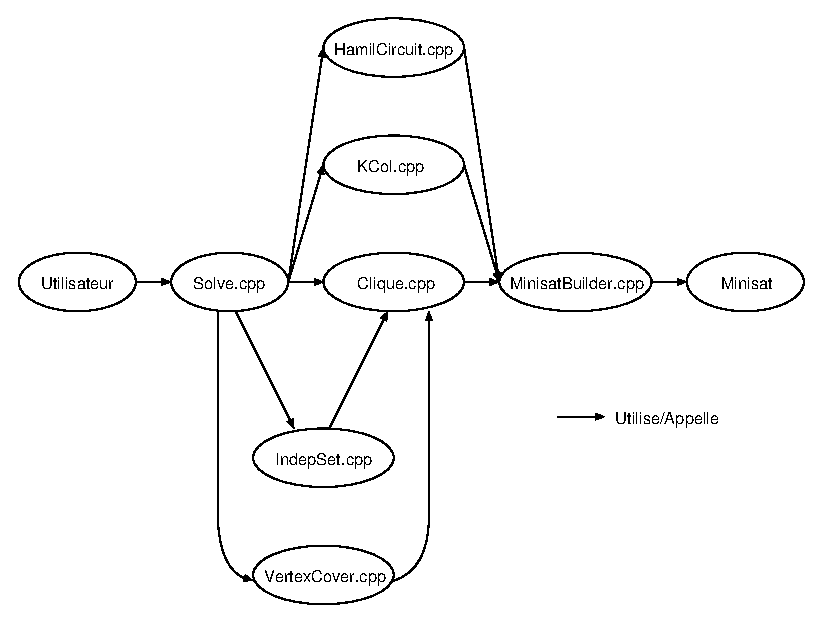
\includegraphics{images/grapheExec.eps}
    \caption{Relations entre les différentes parties du
    programme\label{grapheExec}}
   \end{center}
  \end{figure}

  \subsection{Extension des fichiers}
  Étant donné que nous générons des fichiers avec notre programme, nous
  avons aussi choisi des noms et extensions différentes selon le but du
  fichier.

  En effet nous avons introduit trois extensions différentes :
  \begin{enumerate}
   \item \emph{graph.gin} $\leadsto$ Fichier graphe de type
	 \emph{gengraph} passé en paramètre par l'utilisateur au
	 programme
   \item \emph{graph.sat} $\leadsto$ Fichier qui contient la formule de
	 type \emph{CNF\footnote{Conjunctive Normal Form}} générée par
	 notre programme à partir du choix du problème et du graphe.
   \item \emph{graph.sol} $\leadsto$ Fichier qui contient la solution
	 retournée par \emph{minisat}.
  \end{enumerate}

  Nous avons fait le choix de laisser ces fichiers sur le disque après
  exécution du programme, dans le cas où l'utilisateur souhaiterait y
  jeter un \oe{}il\footnote{Les utilisateurs que nous sommes ont
  beaucoup apprécié cette possibilité.}.

 \section{Idées des réductions}
 Nous allons dans cette partie vous présenter très brièvement les idées
 de réductions que nous avons utilisées. Nous allons seulement citer les
 quelques propriétés caractérisant nos problèmes qui nous ont permis de
 générer les formules \emph{CNF}.
 
 Nous citerons aussi ce que nous avons appelé les ``cas
 faciles'', c'est à dire les cas où nous n'avons pas besoin de
 \emph{Minisat} pour répondre à nos problèmes (problème de décision).

  \subsection{\emph{K-Col} $\leq_P$ \emph{SAT}}
  \underline{Propriétés caractérisant \emph{K-Col} :}
  \begin{enumerate}
   \item Chaque sommet est colorié.
   \item Il n'y a qu'une seule couleur par sommet.
   \item Deux sommets qui se suivent n'ont pas la même couleur.
  \end{enumerate}

  \underline{Cas faciles :}
  \begin{enumerate}
   \item Le nombre de couleurs est négatif.
   \item Le nombre de couleurs est supérieur au nombre de sommets.
  \end{enumerate}

  \subsection{\emph{Circuit Hamiltonien} $\leq_P$ \emph{SAT}}
  \underline{Propriétés caractérisant \emph{Circuit Hamiltonien} :}
  \begin{enumerate}
   \item Chaque noeud est dans le circuit.
   \item Un noeud a exactement une position dans le circuit sauf pour le
	 premier/dernier.
   \item Deux sommets non voisins ne peuvent pas se suivre dans le
	 circuit.
   \item Deux sommets n'ont pas la même position dans le circuit.
   \item Le dernier sommet du circuit doit aussi être le premier.
  \end{enumerate}

  \underline{Cas faciles :}
  \begin{enumerate}
   \item Le nombre d'arêtes du graphe est strictement inférieur au
	 nombre de sommets $\Rightarrow$ Impossible.
   \item Le graphe est un graphe complet $\Rightarrow$ Toujours vrai.
  \end{enumerate}

  \subsection{\emph{Clique} $\leq_P$ \emph{SAT}}
  \underline{Propriétés caractérisant \emph{Clique} :}
  \begin{enumerate}
   \item Chaque noeud est dans la clique.
   \item Un noeud a exactement une position dans la clique.
   \item Deux sommets non voisins ne peuvent pas être ensemble dans la
	 clique.
   \item Deux sommets n'ont pas la même position dans la clique.
  \end{enumerate}

  \underline{Cas faciles :}
  \begin{enumerate}
   \item \emph{Clique} de taille négative $\Rightarrow$ Erreur en
	 entrée.
   \item \emph{Clique} de taille 0 $\Rightarrow$ Toujours vrai.
   \item \emph{Clique} de taille 1 $\Rightarrow$ Nécessite 1 seul
	 sommet.
   \item \emph{Clique} de taille 2 $\Rightarrow$ Nécessite 1 seule
	 arête.
   \item \emph{Clique} de taille strictement supérieure au nombre de
	 sommets $\Rightarrow$ Impossible.
   \item A partir d'un certain nombre d'arêtes par rapport à un nombre
	 de sommets, il est obligatoire d'obtenir une clique d'une
	 certaine taille.
   \item Il faut un nombre d'arêtes minimum pour former une clique d'une
	 certaine taille.
  \end{enumerate}

  \subsection{\emph{Ensemble indépendant} $\leq_P$ \emph{SAT}}
  \underline{Propriétés caractérisant \emph{Ensemble Indépendant} :}
  \begin{enumerate}
   \item Inutiles car il y a une équivalence pour Ensemble indépendant
	 de taille $k$ sur $G = (V,E)$ et \emph{Clique} de taille $k$
	 sur $\overline{G}$ (Réduction de \emph{Ensemble Indépendant} à
	 \emph{Clique}).
  \end{enumerate}

  \underline{Cas faciles :}
  \begin{enumerate}
   \item \emph{IS\footnote{\emph{Independant Set}}} de taille négative
	 $\Rightarrow$ Erreur.
   \item \emph{IS} de taille $0$ $\Rightarrow$ Toujours vrai.
   \item \emph{IS} de taille $1$ $\Rightarrow$ Nécessite 1 seul sommet.
   \item \emph{IS} de taille strictement supérieure au nombre de sommets
	 $\Rightarrow$ Impossible.
   \item On a forcément un \emph{IS} d'une certaine taille si le nombre
	 d'arêtes est trop faible.
   \item Pour que $k$ sommets puissent former un \emph{IS} dans un
	 graphe de taille $n$, il ne faut pas que le nombre d'arêtes
	 dépasse un certain nombre.
  \end{enumerate}

  \subsection{\emph{Couverture par sommets} $\leq_P$ \emph{SAT}}
  \underline{Propriétés caractérisant \emph{Couverture par sommets} :}
  \begin{enumerate}
   \item Inutiles car il y a une équivalence pour \emph{Couverture par
	 sommets} de taille $k$ sur $G = (V,E)$ et \emph{Clique} de
	 taille $|V|-k$ sur $\overline{G}$ (Réduction de
	 \emph{Couverture par sommets} à \emph{Clique}).
  \end{enumerate}

  \underline{Cas faciles :}
  \begin{enumerate}
   \item \emph{VC\footnote{\emph{Vertex Cover}}} de taille négative
	 $\Rightarrow$ Erreur.
   \item \emph{VC} de taille $0$ $\Rightarrow$ Vrai s'il n'y a aucune
	 arête.
   \item \emph{VC} de taille strictement supérieure au nombre de sommets
	 $\Rightarrow$ Impossible.
   \item Pour que k sommets puissent représenter une \emph{VC} dans un
	 graphe de taille $n$, il ne faut pas que le nombre d'arêtes
	 dépasse un certain nombre.
  \end{enumerate}


 \section{Tests et résultats}
  Pour vérifier le bon fonctionnement de notre programme, nous avons
  effectué plusieurs tests qui nous ont permis de nous rendre compte de
  plusieurs problèmes.

  \subsection{Tests}
  Nous avons fait plusieurs tests sur différents types de fichiers
  d'entrée. Ces fichiers tests sont disponibles dans le répertoire
  \emph{jeux}. \newline
  \indent Nous avons testé notre programme sur des fichiers vides,
  et différents types de graphes. Des graphes à une seule arête, et des
  graphes générés par le programme \emph{gengraph}: une clique à 100
  sommets (graphe complet), un chemin à 100 sommets, un graphe aléatoire
  de 100 sommets, un arbre à 100 sommets...

  \subsection{Résultats des tests}
  Ces tests nous ont permis de mettre en avant quelques erreurs de
  programmation que nous avons corrigées mais surtout de trouver des cas
  simples, dont nous avons parlés précédemment, et de voir les limites
  des réductions et de \emph{minisat}.
  \begin{enumerate}
   \item \emph{Circuit Hamiltonien:} Si on lançait la recherche d'un
	 Circuit Hamiltonien sur un graphe complet, à cause du grand
	 nombre de clauses, le temps d'exécution de \emph{minisat}
	 explosait alors qu'il n'y a rien de plus simple à trouver. Cas
	 que nous avons résolu (en ajoutant un cas facile), mais si on
	 enlève une arête à un graphe complet le problème perciste.
   \item \emph{Couverture par sommets:} Si on lance cette réduction sur
	 un graphe de type chemin de taille 100 et que l'on cherche une
	 couverture de sommet de taille 50 ou inférieur (qui n'est pas
	 satisfaisable dans ce denier cas) le temps d'exécution explose
	 littéralement alors qu'en TD, nous avons vu que, pour ce genre
	 de graphe et pour un nombre de sommet paire $n$, la plus petite
	 couverture de sommet est de taille $n/2$ (voir \ref{an1} page
	 \pageref{an1} en annexe).
  \end{enumerate}

  \indent Sur des graphes de taille correcte à l'échelle papier (i.e. 4
  ou 5 sommets), les résulats ont tous été concluant. Le résultat de
  l'exécution du programme pour un \emph{Circuit Hamiltonien} (\ref{ham}
  page \pageref{ham}) sur le graphe \ref{graphe1} page \pageref{graphe1} 
  (voir aussi \ref{an2} page \pageref{an2} en annexe pour KCol)
  est bien un \emph{Circuit Hamiltonien}.

  \begin{figure}[!ht]
   \begin{center}
    \includegraphics[height=5cm]{images/jeurap.ps}
    \caption{Graphe de test jeurapport.gin .\label{graphe1}}
   \end{center}
  \end{figure}

  \begin{figure}[!ht]
   \begin{center}
    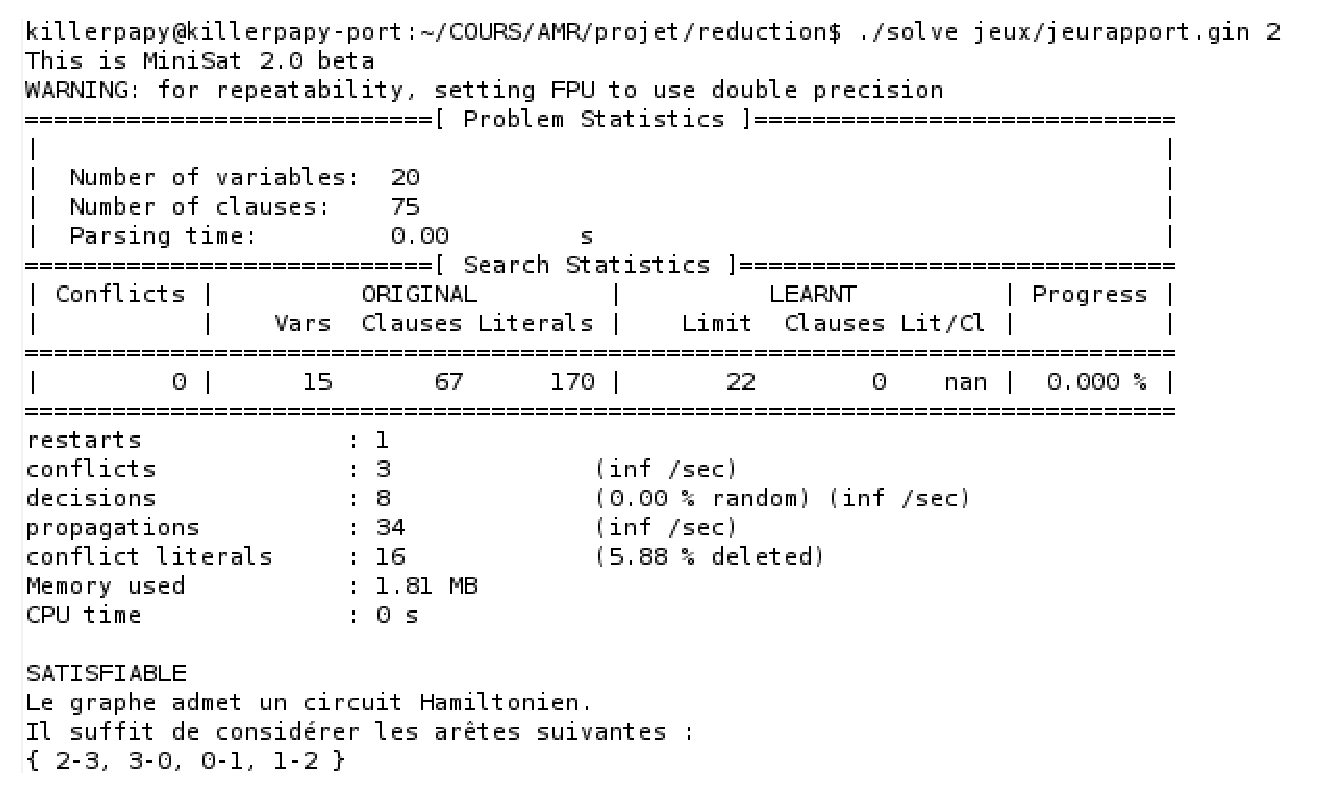
\includegraphics[width=12cm]{images/chemin.eps}
    \caption{\emph{Circuit Hamiltonien} sur le graphe
    \ref{graphe1}.\label{ham}}
   \end{center}
  \end{figure}
\input{difficulties}
% -*- mode: latex; coding: latin-1-unix -*- %
\section{Bilan}

\subsection{Difficultées rencontrées}

\subsubsection{Problématique du damier}

Nous avions initialement prévu que la mission se déroulerait dans un environnement ou le sol serait homogène (exemple: tout blanc). Cependant, un problème de décision est survenu. Il était impossible de différencier la présence de l'absence d'un chemin à gauche ou à droite lors de la rencontre d'un obstacle. Etant donné que le robot reste sur la même case lors de sa rotation, il aurait fallu décider d'une distance ou durée avant la rencontre potentielle d'un nouvel obstacle sur le nouveau chemin, ce qui va à l'encontre  de l'objectif de réactivité et généricité du comportement du robot. Pour éviter de temporiser cette action, nous avons décidé d'utiliser un damier gris et blanc, permettant de décider au premier changement de case sur le nouveau chemin si ce chemin est effectivement utilisable ou si la solution était la direction opposée (rencontre immédiate d'une nouvelle case noire).

\subsubsection{Calibrage du capteur lumineux}

Selon les différentes intensités lumineuses dans la pièce où se trouve le robot, les bornes des 3 seuils utilisés doivent être adaptées. Tout au long du projet, il a fallu ajuster ces valeurs de manière à ce que le robot détecte bien les différentes couleurs de cases et à ce que les prises de décision ne soient pas faussées. Il était parfois difficile de faire la différence entre un bug logique (erreur dans le code) et un bug physique (intéractions avec l'environnement). Nous estimons que les bornes sont actuellement positionnées de manière à rendre la mission possible dans un maximum d'endroits et de luminosités différentes.

\subsubsection{Problématique de seuil intermédiaire du capteur lumineux}

Lors du passage du capteur entre les 2 seuils extrêmes (case blanche à case noire ou case noire à case blanche), le capteur détecte un seuil intermédiaire gris pendant un bref instant, causant un bug dans la prise de décision. Nous avons du mettre en place un procédé de correction de la detection qui renouvelle la lecture du capteur après un très bref instant et change la valeur obtenue si elle est différente de la dernière lecture. Cette temporisation était incontournable.

\subsubsection{Caractère incontrolable des valeurs retournées par les capteurs}

Au début de notre modélisation Altarica des capteurs, nous pensions pouvoir nous en sortir avec une variable d'état $value$ pour représenter les valeurs "lues" par le capteur de lumière et le capteur ultrasonique. Et un évenement $readValue$ devait survenir en fonction de chaque changement de valeur de notre variable d'état. Cela ne convenait pas ensuite dans la vérification, car en réalité, il est impossible de prévoir les valeurs qui vont \^{e}tres lues par ces capteurs. Le robot est réactif à son environnement. Nous avons donc remplacés ces modélisations par une simple variable de flux, qui est bien incontrolable et donc cohérente.

\subsubsection{Possibilité de tirer des transitions non voulues}

Au moment de simuler notre n\oe{}ud Controller, nous avons remarqué qu'il nous était possible de faire tourner le robot maître à droite, alors qu'en réalité, cela ne correspondait pas. Nous avons ensuite compris qu'il s'agissait d'une action non capturée d'un sous-n\oe{}ud de notre Controller. Nous avons donc remarqué que cet événement n'était pas capturé parce que le robot maître ne tournait jamais à droite.

\subsection{Conclusion}

Nous avons apprécié l'approche que nous avons eue pendant ce projet. Nous ne nous sommes pas uniquement concentrés sur des difficultés logicielles, et avons abordés les problèmes techniques découlant d'un système complet (électronique et logiciel). Nous aurions voulu aller au bout de notre démarche mais le temps nous a manqué.

Il nous semble que la réalisation d'un outil de génération de code automatique, reposant sur notre travail, est tout à fait envisageable en utilisant une méthode proche de celle que nous avons proposée.


%%%%%%               %%%%%%
%%%%%% /ZONE DE CODE %%%%%%
%%%%%%               %%%%%%

\end{document}

%%%%%%           %%%%%%
%%%%%% /DOCUMENT %%%%%%
%%%%%%           %%%%%%




%%%%% Texte italique %%%%%
%  \textit{} 

%%%%% Liste %%%%
%%% Itemize %%%
%  \begin{itemize}
%   \item item1\\
%   \item item2
%  \end{itemize}

%%% Enumerate %%%
%  \begin{enumerate}
%   \item item1
%   \item item2
%  \end{enumerate}

%%%%% Tabulations %%%%%
%   \begin{tabbing}
%    XX\=XX\=\kill
%    \>(OrdresEnonce.v, ligne 244)\\
%    \>\>test2
%   \end{tabbing}
 
%%%%% Note de pied de page %%%%%
%  \footnote{test}

%%%%% Référence %%%%%
%   \label{ref}
%% Plus loin :
%   \ref{ref}
%   \pageref{ref}

%%%%% Code %%%%%
% \begin{lstlisting}
%      List<Integer> lexBFS2 = new ArrayList<Integer>();
%      lexBFS2.add(3);
%      lexBFS2.add(2);
%      lexBFS2.add(4);
%      lexBFS2.add(1);
%      lexBFS2.add(0);    
%      assertNotNull(lexBFS2);	
%      assertEquals(lexBFS2,Graphs.lexBFS(nogYComp));
%   \end{lstlisting}

%%%%% Figure %%%%%
%  \begin{figure}[!ht]
%   \begin{center}
%	\includegraphics[width=7cm]{figs/cours1/fig2.eps}
%	\caption{\emph{MT2} : Calcul non déterministe}
%   \end{center}
%  \end{figure}
